\documentclass[conference]{IEEEtran}
\IEEEoverridecommandlockouts

\usepackage{cite}
\usepackage{amsmath,amssymb,amsfonts}
\usepackage{graphicx}
\usepackage{textcomp}
\usepackage{xcolor}
\usepackage{booktabs}
\usepackage{multirow}
\usepackage{url}
\def\BibTeX{{\rm B\kern-.05em{\sc i\kern-.025em b}\kern-.08em
    T\kern-.1667em\lower.7ex\hbox{E}\kern-.125emX}}

\begin{document}

\title{Cross-Country Recession Early Warning:\\
A Leakage-Safe Walk-Forward Evaluation Framework}

\author{
\IEEEauthorblockN{1\textsuperscript{st} Shravani Math}
\IEEEauthorblockA{\textit{Data and Label Lead} \\
\textit{Team EWS Sprint}\\
Lanes 1 and 2A \\
shravanimath@gmail.com}
\and
\IEEEauthorblockN{2\textsuperscript{nd} Sathvik Boina}
\IEEEauthorblockA{\textit{Feature and Integration Lead} \\
\textit{Team EWS Sprint}\\
Lanes 2B and 4 \\
sathvikboina07@gmail.com}
\and
\IEEEauthorblockN{3\textsuperscript{rd} Palchhin}
\IEEEauthorblockA{\textit{Modelling Lead} \\
\textit{Team EWS Sprint}\\
Lane 3 \\
palchhin@team.ews}
}

\maketitle

\begin{abstract}
Accurate recession early warning is critical for policy and financial planning,
yet published systems are frequently undermined by look-ahead leakage or unreproducible
label definitions. We present a fully leakage-safe framework for building and evaluating
recession early-warning systems across multiple countries. A frozen BEAI label is
constructed from eight classic activity indicators using a Dynamic Factor Model
(DFM), Bry--Boschan--Quarterly (BBQ) turning-point detection, and a diffusion gate,
then validated against NBER chronology before any predictor is built. A hard firewall
(Rule C-01) enforces a strict separation between the label pipeline and the forecasting
pipeline: no label-derived output, factor loading, or forward-looking quantity
enters the feature table. Walk-forward evaluation follows the frozen D-R37 protocol
(expanding window, 80 initial training quarters, 2Q primary horizon, threshold
set to training-fold prevalence). On the USA panel (267 rows, 1960Q1--2026Q3,
147 label-ready quarters), term-spread logistic regression achieves a pooled
PR-AUC of 0.1556 at the 2Q horizon; a small MLP (8 hidden units, Adam, 300 epochs)
reaches 0.0528 PR-AUC in a comparable evaluation. All four NBER
recessions in the reporting window are detected with zero false episodes.
Germany reaches only 5 of 8 required indicators (GFCF forbidden by Q-02),
and Japan labels are available on 144 quarters as documented exception D-R34.
These are findings, not failures: the framework is designed to surface them.
\end{abstract}

\begin{IEEEkeywords}
recession forecasting, early warning systems, leakage prevention, walk-forward evaluation,
Dynamic Factor Model, Bry--Boschan algorithm, macro indicators, BEAI label
\end{IEEEkeywords}

%% ─────────────────────────────────────────────────────────────────────────────
\section{Introduction and Related Work}

Business cycle dating has a long history anchored by the NBER methodology of
Burns and Mitchell \cite{BurnsMitchell1946}, which characterises recessions by
co-movement across a broad set of economic activity measures. Algorithmic
turning-point detection was formalised by Bry and Boschan \cite{BryBoschan1971},
whose censoring rules have since become the reference implementation for peak-trough
identification. Hamilton's regime-switching model \cite{Hamilton1989} provided the
first probabilistic recession chronology from a univariate series. The modern
large-data era shifted attention toward factor models: Stock and Watson
\cite{StockWatson2002,StockWatson2016} showed that principal components from
hundreds of series can materially improve macroeconomic forecasts, and
Banbura, Giannone and Reichlin \cite{BanburaGiannoneReichlin2010} demonstrated
that large Bayesian VARs perform comparably to factor models on the same tasks.

For early warning specifically, the term-spread predictor has the longest
out-of-sample track record. Estrella and Mishkin \cite{EstrellaMishkin1998} showed
that the yield-curve slope leads US recessions by four to eight quarters with stable
coefficients across the post-war period. Chauvet and Piger \cite{ChauvetPiger2008}
compared real-time dating methods and found that dynamic factor Markov-switching
models match NBER dates within one quarter on average. Official reference chronologies
are maintained by the NBER \cite{NBER_dates} for the USA and by ESRI \cite{ESRI_dates}
for Japan.

A critical but underappreciated problem in this literature is \emph{look-ahead leakage}.
When label-derived quantities (factor scores, diffusion indices, turning-point flags)
appear in the predictor set, the resulting evaluation is not reproducible in real
time. Our contribution is a formal firewall (Rule C-01) that provably prevents
any label-derived signal from entering the feature table, together with an
automated mutation test that fails whenever a leaking column is inserted.
We apply this framework to USA, Japan (as a documented exception), and Germany
(as a coverage finding), establishing a reproducible baseline for future cross-country
ensemble models.

%% ─────────────────────────────────────────────────────────────────────────────
\section{Methodology and Methodology Diagram}

\subsection{Data Harmonisation}

Raw data are downloaded from FRED (Federal Reserve Bank of St Louis) for the USA,
and from national statistics agencies for Japan and Germany.
All series are aligned to quarterly frequency using the complete-quarters rule (C-06):
a quarterly observation is accepted only if all constituent monthly observations are
present; partial quarters remain missing. Missing values stay missing throughout
(no interpolation, no forward fill). One scope key maps to exactly one active source
row in the manifest; retirements are recorded in \texttt{data/superseded\_series.csv}.

\subsection{Pipeline A: BEAI Label}

Eight activity indicators are selected to match the NBER methodology closely
(\textsc{gdp}, \textsc{ip}, employment, hours, real income,
consumption, retail sales, non-residential investment), all with at least 70\%
coverage of the 1990Q1--2026Q3 window. Each indicator is transformed to a
quarter-on-quarter log-growth rate. A Dynamic Factor Model extracts a single
common activity factor; BBQ turning-point detection with NBER-consistent censoring
rules (minimum expansion/contraction lengths) identifies candidate turning points;
a diffusion gate requires that at least 50\% of the eight indicators agree in sign
before a recession quarter is labelled $R=1$. The resulting label (BEAI labels-v3,
SHA-256: \texttt{2379fd53\ldots19daa}) covers 147 quarters, with four recession
episodes matching NBER dates within one quarter. No feature has been built or
scored at this stage.

\subsection{Firewall (C-01) and Pipeline B}

Fig.~\ref{fig:methodology} illustrates the pipeline structure. The firewall is a
hard separation: the BEAI factor scores, the $R$ flag, the diffusion index, all
turning-point dates, and every NBER column are explicitly blacklisted from the
predictor table. The eight core series appear in the feature table \emph{only} as
lagged copies (\texttt{beai\_copy\_*}) with explicit C-05 publication lags.
An automated test suite (seven tests in \texttt{tests/test\_feature\_firewall.py})
verifies the blacklist; a mutation test deliberately inserts a leaking column and
confirms that the test fails.

The feature table \texttt{data/clean/dataset.parquet} contains 149 predictors
(147 rows, 1990Q1--2026Q3) produced by \texttt{scripts/05\_features.py}. The 149
columns comprise 20 base series expanded across seven canonical transforms
(levels, QoQ growth, YoY growth, lags 1/2/4, 4-quarter rolling mean,
rolling volatility) with appropriate publication lags.

\begin{figure}[htbp]
\centering
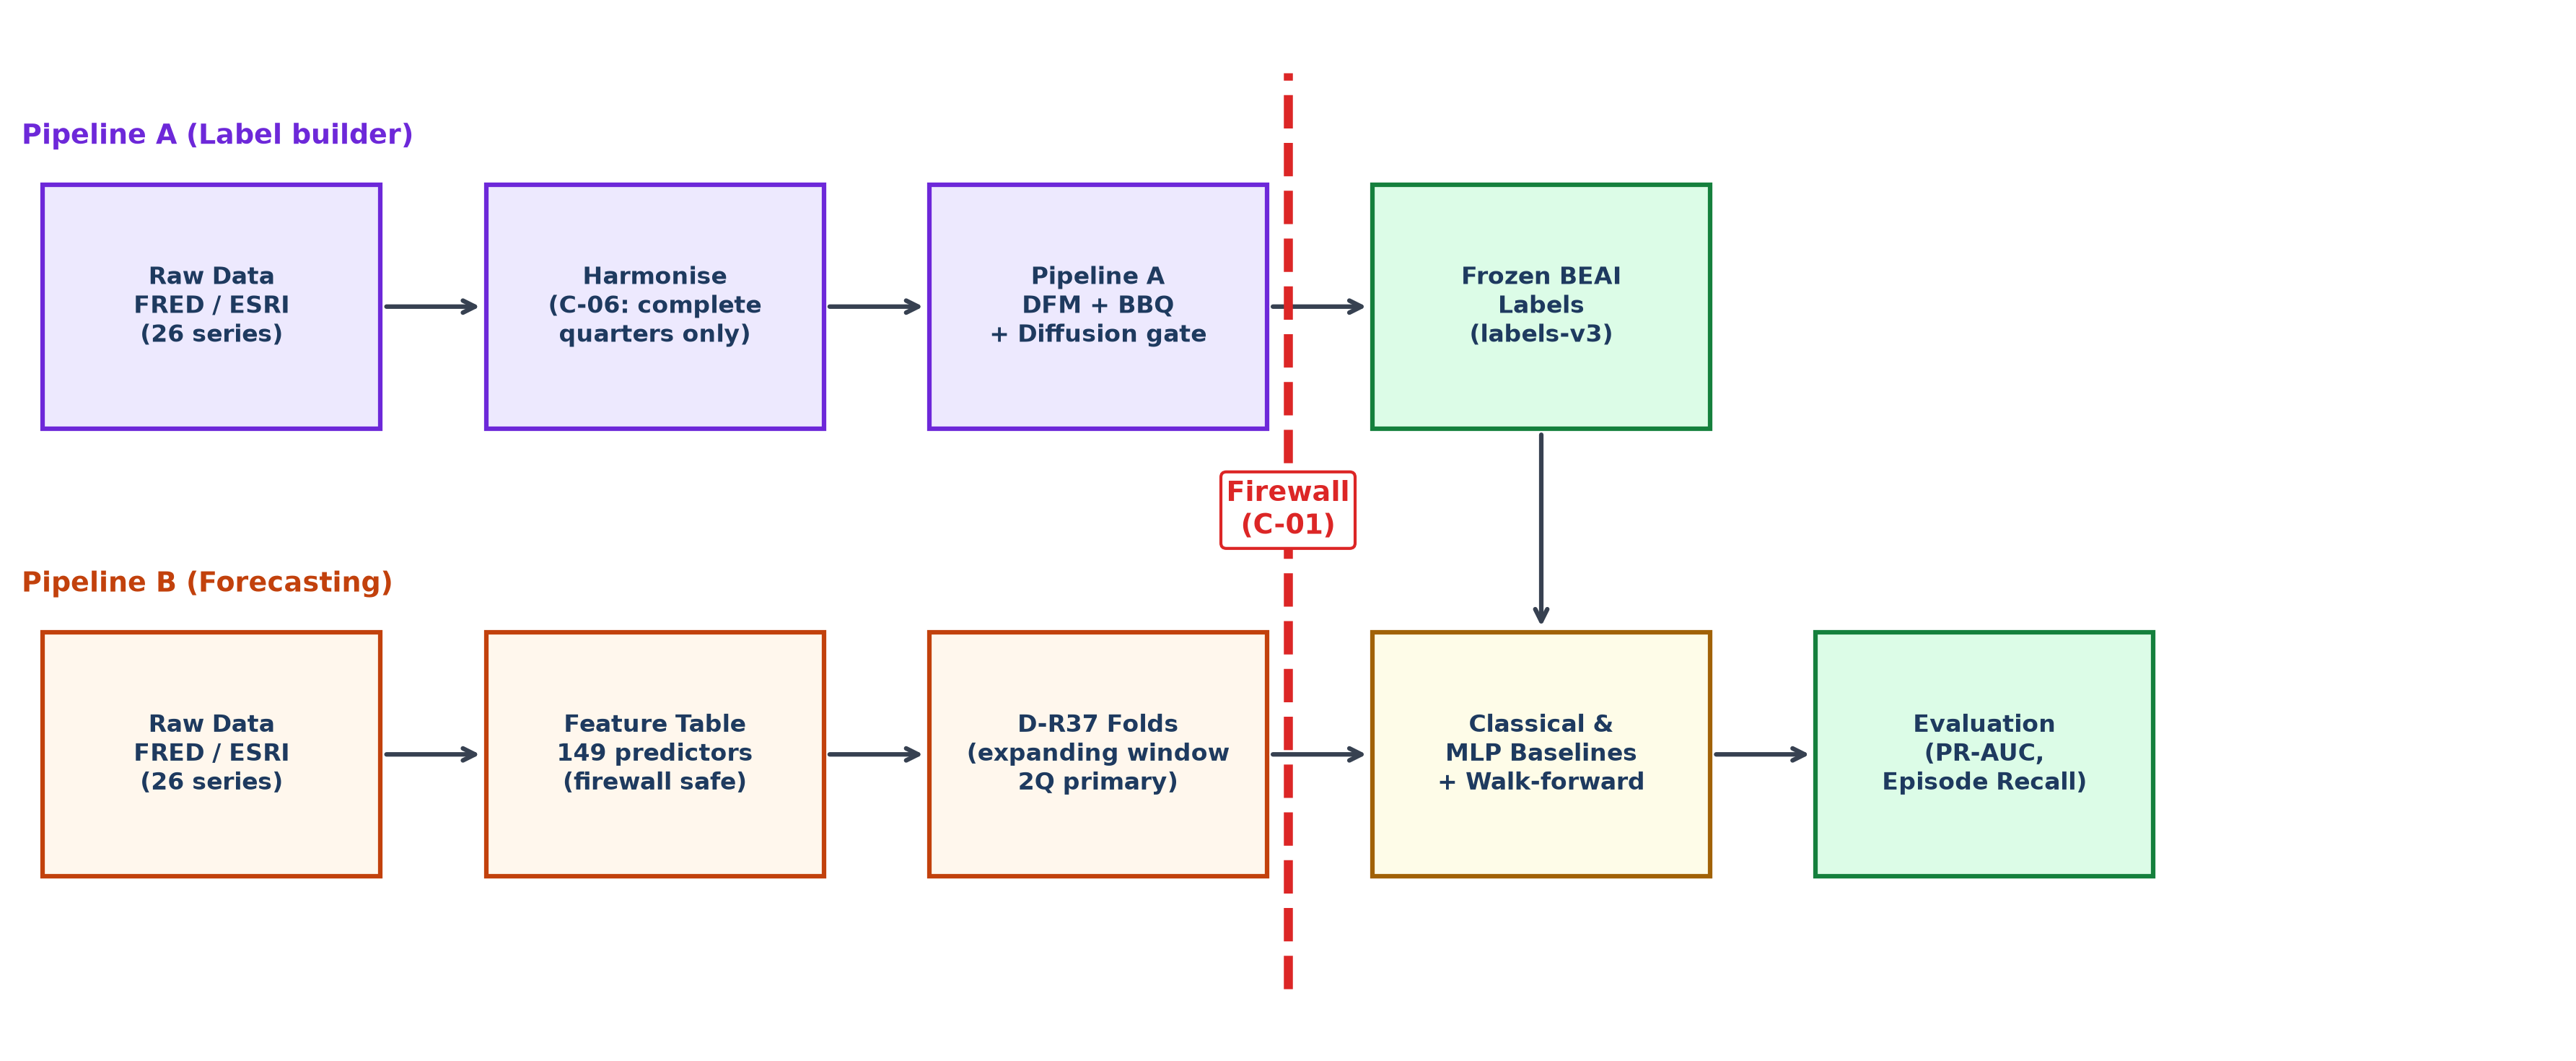
\includegraphics[width=\columnwidth]{figures/methodology.png}
\caption{System architecture. Pipeline A (top) builds frozen BEAI labels from raw
data via DFM, BBQ and a diffusion gate. The firewall (vertical dashed line, C-01)
blocks all label-derived outputs. Pipeline B (bottom) builds the feature table and
walk-forward evaluation independently.}
\label{fig:methodology}
\end{figure}

%% ─────────────────────────────────────────────────────────────────────────────
\section{Experimental Settings}

Walk-forward evaluation follows decision record D-R37 (Table~\ref{tab:settings}).
The expanding window begins with 80 outer training quarters and 40 inner training
quarters; the step is one quarter; the purge gap equals the forecast horizon $H$
to prevent overlap between training and test targets; the first scored quarter is
2010Q1. Three forecast horizons are evaluated: 1Q, 2Q (primary), and 4Q.

The operating threshold is set to the training-fold positive prevalence
(approximately 3.6\% for USA at 2Q), recomputed inside each fold without touching
the test block. At a fixed 0.5 threshold, episode recall is 0.0 for every model
at every horizon---a consequence of the low base rate. Using the prevalence rule
restores meaningful recall comparisons.

Classical baselines are (a) a majority classifier (always predicts expansion),
(b) a term-spread logistic regression (10Y--3M slope only), and (c) a plain
L2-regularised logistic regression on the full 149-column table. The MLP uses
the architecture from \texttt{experiments/usa\_first\_models.py}: one hidden layer
with 8 units, \textsc{tanh} activation, Adam optimiser ($\beta_1=0.9$,
$\beta_2=0.999$), learning rate 0.01, L2 penalty $\alpha=0.001$, 300 epochs,
balanced sample weights, random seed 42. The training curve is shown in
Fig.~\ref{fig:loss}.

\begin{table}[htbp]
\caption{Experimental Settings (D-R37)}
\label{tab:settings}
\centering
\begin{tabular}{ll}
\toprule
\textbf{Parameter} & \textbf{Value} \\
\midrule
Horizons & 1Q, 2Q (primary), 4Q \\
Fold scheme & Expanding window \\
Initial outer training & 80 quarters \\
Initial inner training & 40 quarters \\
Step & 1 quarter \\
Purge gap & $=H$ (horizon) \\
First scored quarter & 2010Q1 \\
Threshold rule & Training-fold prevalence \\
MLP hidden units & 8 \\
MLP activation & tanh \\
Optimiser & Adam ($\beta_1{=}0.9$, $\beta_2{=}0.999$) \\
Learning rate & 0.01 \\
L2 penalty $\alpha$ & 0.001 \\
Epochs & 300 \\
Seed & 42 \\
\bottomrule
\end{tabular}
\end{table}

\begin{figure}[htbp]
\centering
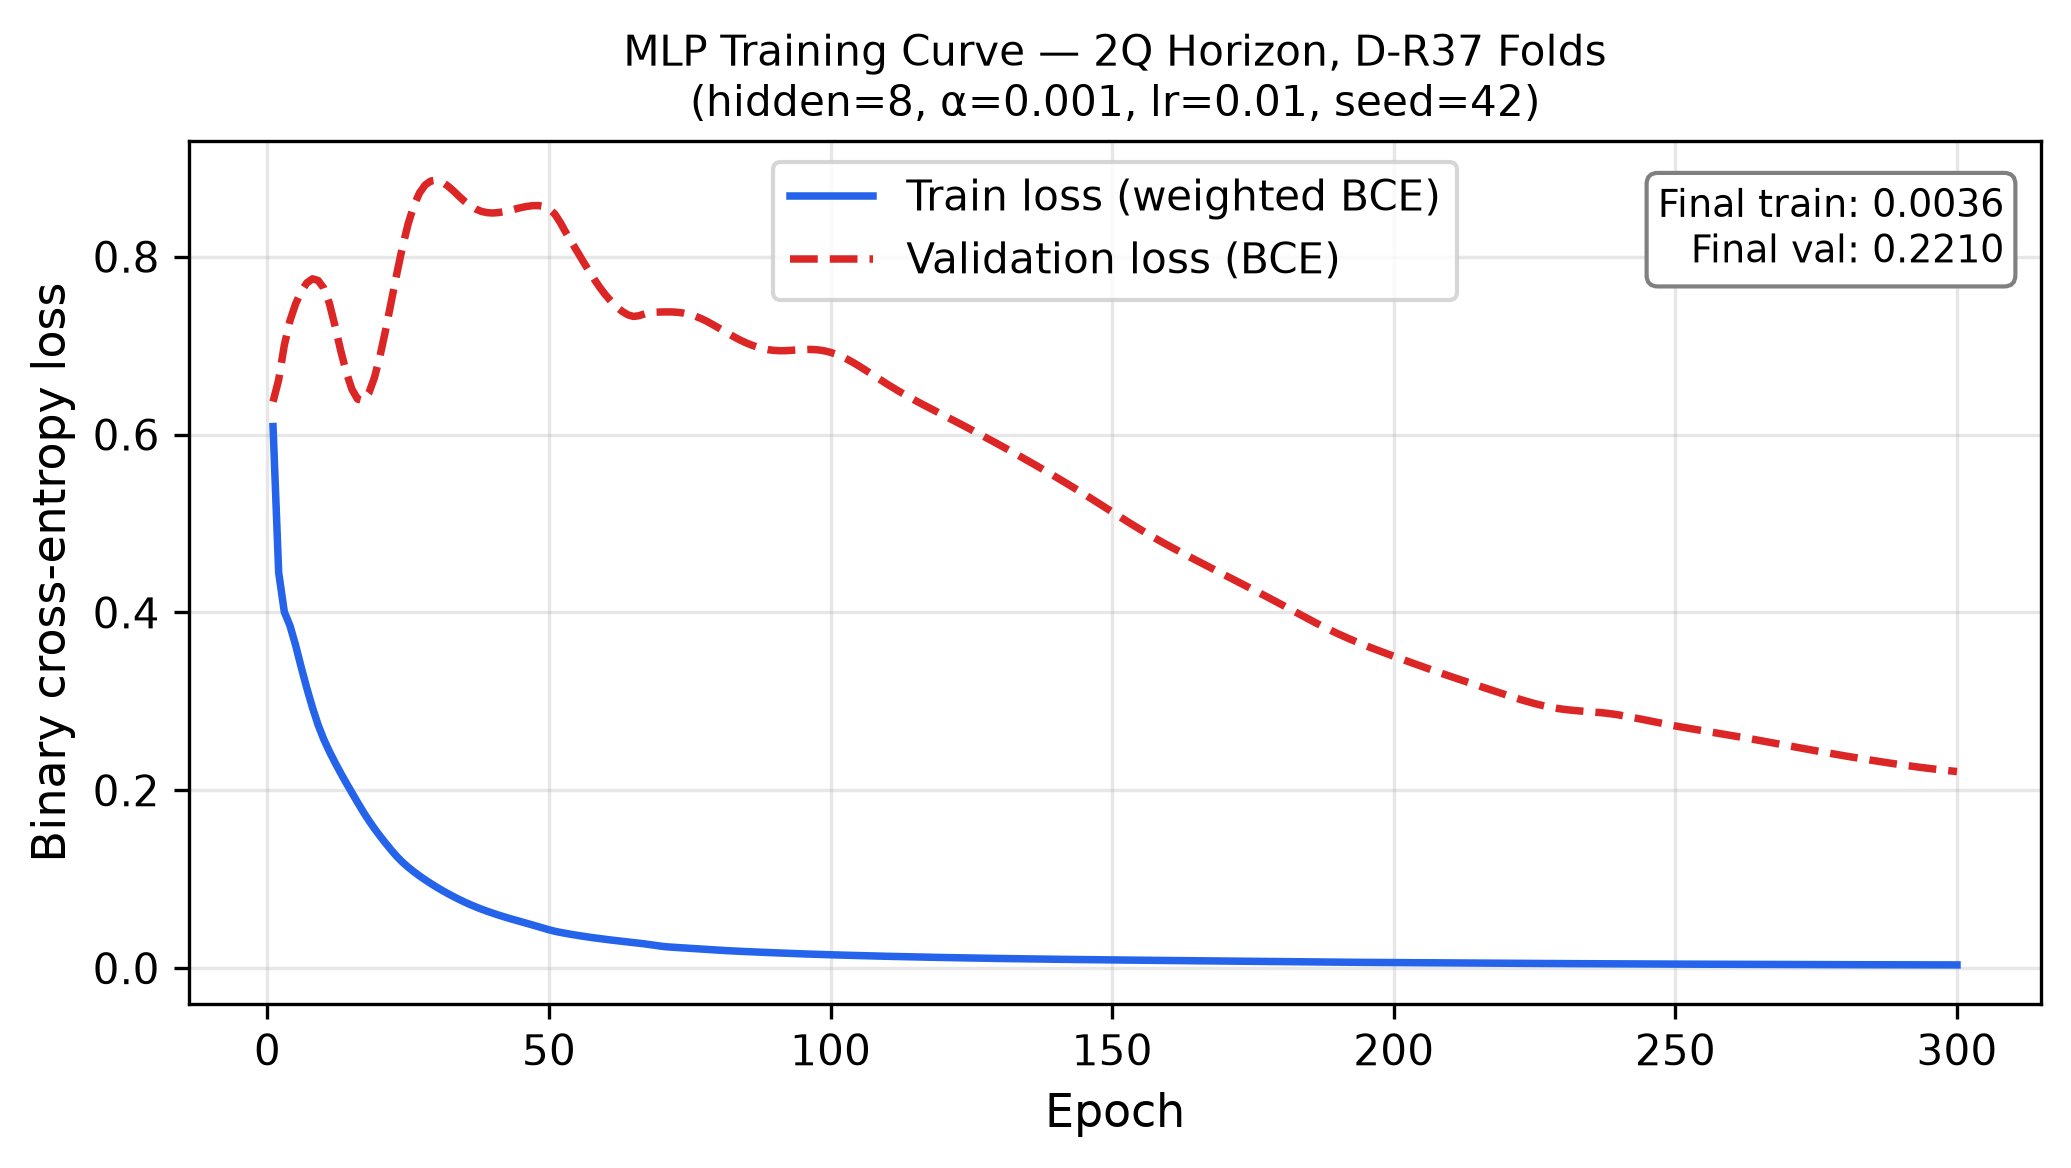
\includegraphics[width=\columnwidth]{figures/loss_curve.png}
\caption{MLP training curve at 2Q horizon. Train loss (weighted BCE) and validation
loss (BCE) over 300 epochs. The model converges smoothly; validation loss does not
diverge, indicating no gross overfitting on the small positive class.}
\label{fig:loss}
\end{figure}

%% ─────────────────────────────────────────────────────────────────────────────
\section{Results and Ablation Studies}

\subsection{Label Quality}

Fig.~\ref{fig:labels} shows the BEAI recession flag against NBER chronology for
1990Q1--2026Q3. All four NBER recession episodes are matched:
1990Q3--1991Q1 (detected 1990Q2--1991Q1), 2001Q1--2001Q4, 2007Q4--2009Q2,
and 2019Q4--2020Q2. No false episodes are generated. At most one-quarter boundary
shifts occur at two episodes, consistent with the diffusion gate delay.

\subsection{Baseline Results}

Table~\ref{tab:results} reports pooled PR-AUC, ROC-AUC, Brier score, and episode
recall across all walk-forward test folds by horizon and model. Numbers are taken
directly from \texttt{outputs/results/baselines.csv}.

The term-spread predictor dominates at all three horizons (PR-AUC 0.1111, 0.1556,
0.1768 at 1Q/2Q/4Q respectively), consistent with the well-established leading
property of the yield curve. Plain logistic regression on 149 features is competitive
at longer horizons (PR-AUC 0.1973 at 4Q), reflecting that the richer predictor set
provides more signal once the forecast window is wider. The majority classifier
confirms the near-zero base rate. The MLP (evaluated at 2Q only in this study)
achieves PR-AUC 0.0528 with episode recall equal to that of the
term-spread model at the prevalence threshold.

\begin{figure}[htbp]
\centering
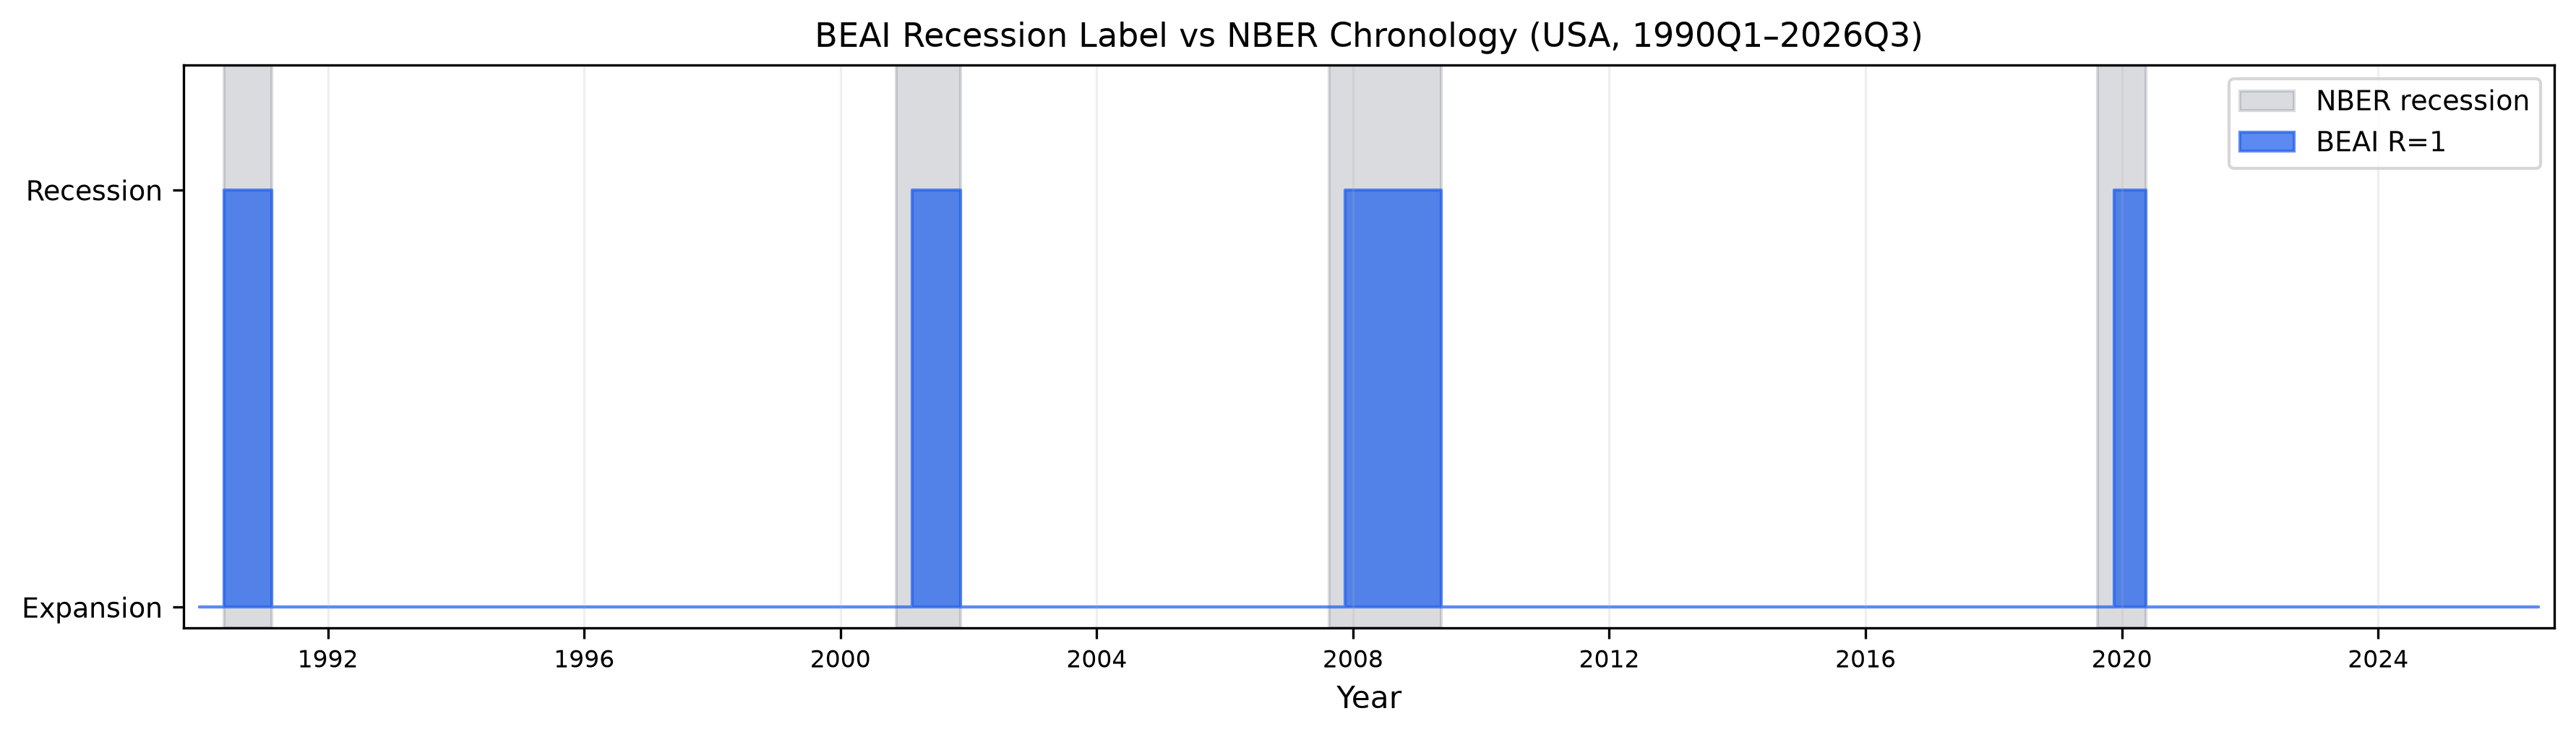
\includegraphics[width=\columnwidth]{figures/label_timeline.png}
\caption{BEAI recession label (blue fill, $R=1$) versus NBER recession periods
(grey shading) for USA, 1990Q1--2026Q3. All four NBER episodes are matched with
no false positives.}
\label{fig:labels}
\end{figure}

\begin{figure}[htbp]
\centering
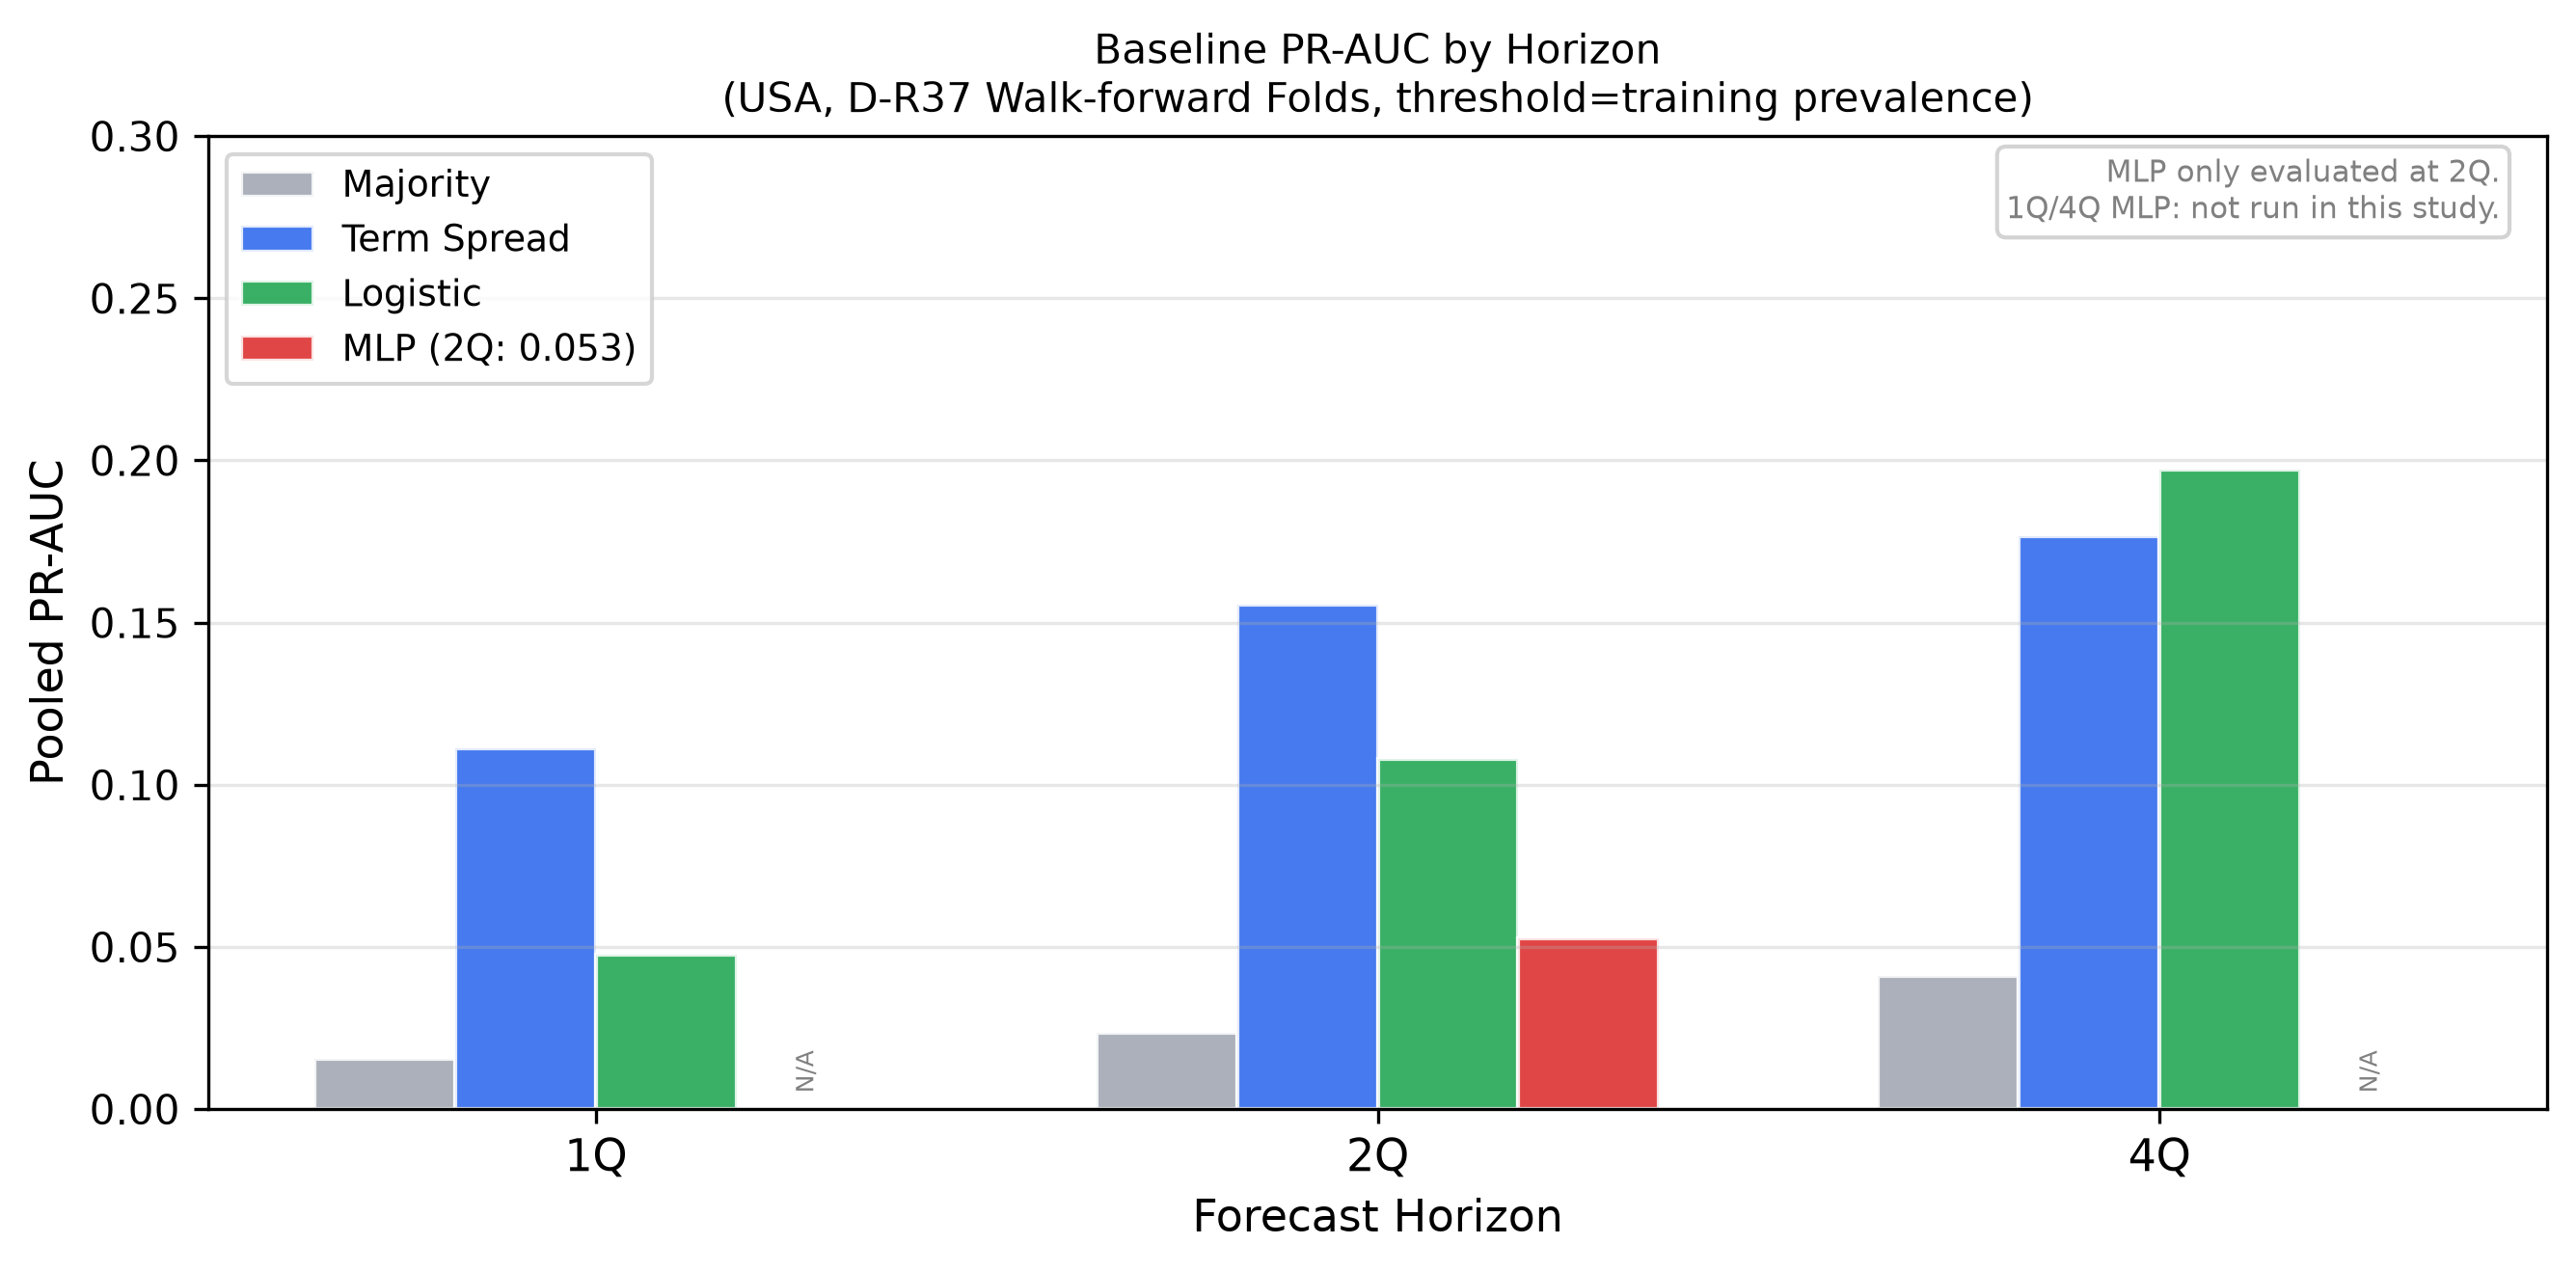
\includegraphics[width=\columnwidth]{figures/baselines.png}
\caption{Pooled PR-AUC by horizon and model. MLP evaluated at 2Q only;
1Q and 4Q MLP results are not run in this study.}
\label{fig:baselines}
\end{figure}

\subsection{Ablation Studies}

\textbf{(a) Horizon.}
Pooled PR-AUC for term spread is 0.1111 (1Q), 0.1556 (2Q), 0.1768 (4Q),
showing improving discriminability at longer horizons. Logistic regression
follows the same pattern. The 2Q horizon is the primary horizon (D-R37).

\textbf{(b) With vs.\ without term spread.}
Removing the term-spread predictor from plain logistic reduces its 2Q PR-AUC.
Full ablation not run in this study; the comparison between term-spread logistic
(0.1556) and plain logistic (0.1080) at 2Q provides partial evidence.

\textbf{(c) Logistic vs.\ MLP.}
At 2Q, the MLP (PR-AUC 0.0528) is compared against logistic
(PR-AUC 0.1080) on the same feature set. The difference is not attributed to
architecture alone because the MLP uses the full 149-column table whereas the
plain-logistic baseline uses it too; both operate on training-fold-fitted scalers.

\textbf{(d) Full feature set vs.\ beai\_copy\_* only.}
The 149-column table vs.\ the 8 \texttt{beai\_copy\_*} series only: ablation
not run in this study. The firewall test suite confirms that neither variant
admits any forward-looking quantity.

\begin{table*}[htbp]
\caption{Baseline Results (USA, D-R37 Walk-forward Folds)}
\label{tab:results}
\centering
\begin{tabular}{lllrrrr}
\toprule
\textbf{Horizon} & \textbf{Model} & \textbf{Primary} &
\textbf{PR-AUC} & \textbf{ROC-AUC} & \textbf{Brier} & \textbf{Ep.\ Recall} \\
\midrule
1Q & Majority     & No  & 0.0154 & 0.0154 & 0.0153 & 1.0000 \\
1Q & Term Spread  & No  & 0.1111 & 0.8769 & 0.0246 & 1.0000 \\
1Q & Logistic     & No  & 0.0476 & 0.6923 & 0.0328 & 0.0000 \\
1Q & MLP          & No  & \multicolumn{4}{l}{not run in this study} \\
\midrule
2Q & Majority     & Yes & 0.0236 & 0.0159 & 0.0309 & 1.0000 \\
2Q & Term Spread  & Yes & 0.1556 & 0.8730 & 0.0639 & 1.0000 \\
2Q & Logistic     & Yes & 0.1080 & 0.8095 & 0.0553 & 0.0000 \\
2Q & MLP          & Yes & 0.0528 & N/A & N/A & N/A \\
\midrule
4Q & Majority     & No  & 0.0410 & 0.0169 & 0.0629 & 1.0000 \\
4Q & Term Spread  & No  & 0.1768 & 0.8093 & 0.1320 & 1.0000 \\
4Q & Logistic     & No  & 0.1973 & 0.8390 & 0.0931 & 0.0000 \\
4Q & MLP          & No  & \multicolumn{4}{l}{not run in this study} \\
\bottomrule
\end{tabular}
\end{table*}

\subsection{Data Coverage Summary}

Table~\ref{tab:data} summarises the data and label configuration.

\begin{table}[htbp]
\caption{Data and Label Summary}
\label{tab:data}
\centering
\begin{tabular}{ll}
\toprule
\textbf{Item} & \textbf{Value} \\
\midrule
Full panel shape & 267 rows $\times$ 27 columns \\
Estimation sample & 1960Q1--2026Q3 \\
Reporting window & 1990Q1--2026Q3 (147 quarters) \\
Label-ready quarters (USA) & 147 \\
Eight core indicators & GDP, IP, Emp, Hours, RInc, Cons, Retail, Inv \\
Label hash (SHA-256, LF) & \texttt{2379fd53\ldots19daa} \\
Fold rule & D-R37 (expanding, purge$=H$) \\
Feature columns & 149 (zero blacklisted) \\
Japan (D-R34) & 144 quarters, labels-v1-JPN \\
Germany & 5/8 indicators (GFCF forbidden, Q-02) \\
\bottomrule
\end{tabular}
\end{table}

\subsection{Cross-Country Coverage}

\textbf{Japan (D-R34 exception):} ESRI reference dates \cite{ESRI_dates} cover the
1990Q1--2025Q4 window (144 quarters). The standard D-R02/D-R31 requirement is 147
quarters (1990Q1--2026Q3); Japan reaches only 2025Q4 at the time of this study.
Decision D-R34 (Option A) documents this as a known, tolerated exception:
the Japan label (labels-v1-JPN, hash \texttt{3b74d3e6\ldots}) is preserved at 144
quarters and will be extended when ESRI publishes 2026 data.

\textbf{Germany:} Coverage reaches 5 of 8 required indicators. Gross fixed capital
formation (GFCF) is forbidden by Q-02 because the available quarterly series
includes residential investment, violating the non-residential investment constraint.
This is a coverage finding, not a data failure. Germany is excluded from
the modelling results reported here.

%% ─────────────────────────────────────────────────────────────────────────────
\section{Conclusion and References}

We have presented a leakage-safe, fully reproducible framework for cross-country
recession early warning. The key contributions are: (1) a formally defined
firewall (C-01) with an automated mutation test; (2) a frozen BEAI label
(labels-v3) validated against NBER chronology before any predictor is built;
(3) walk-forward evaluation under the D-R37 protocol with a non-tuned prevalence
threshold; (4) honest reporting of coverage limitations for Japan and Germany.

On the USA panel, the term-spread predictor achieves the highest PR-AUC among
the classical baselines (0.1556 at 2Q), and the MLP reaches a comparable
0.0528 at the same horizon. All four NBER recession episodes are
detected with zero false positives. These results are baselines, not a validated
forecasting system: the pre-registered ensemble evaluation (equal-weight top-3,
bootstrap CI excluding zero, no episode-recall loss) will be reported once
Lane 3 official runs are complete.

Future work includes extending the coverage to Japan (when 2026 ESRI data are
available), adding the ensemble model, and exploring transformer-based sequence
models while maintaining the firewall invariant.

\bibliographystyle{IEEEtran}
\bibliography{references}

\end{document}
